\chapter{Les structures arborescentes}
\minitoc
Nous allons voir deux types d'arbres : 
\begin{enumerate}
	\item L'arbre GRD : << Gauche Racine Droite >>
	\item Les arbres rouges noirs
\end{enumerate}
Ce sont des arbres binaires: chaque noeud de l'arbre à au lu deux fils. 
\attention{Les informations sont rangés dans l'arbre en respectant un certain critère}
\section{L'arbre GRD : <<Gauche Racine Droite>>}
	\subsection{Critère de rangement}
	Quelque soit le noeud de l'arbre : 
	\begin{itemize}
		\item les informations rangées à gauche de la racine de ce noeud sont inférieur ou égal à cette racine.
		\item les informations rangées à droite de la racine de ce noeud sont supérieur à cette racine.
	\end{itemize}
\begin{figure}[H]
\centering
\includegraphics[width=6cm]{content/schemas/arbresGRB.eps}
\caption{Arbre GRB}
\end{figure}
Cet arbre est prévu pour effectuer un parcours en profondeur.
	\subsection{Implémentation du TAD}
\begin{figure}[H]
\centering
\includegraphics[width=10cm]{content/schemas/arbresGRBImplementation.eps}
\caption{Implémentation de l'arbre GRB}
\end{figure}
\lstinputlisting[language=C, caption=Arbre GRD -- Header]{content/code/arbreGRB.h}
\lstinputlisting[language=C, caption=Arbre GRD -- Implémentation]{content/code/arbreGRB.c}

\subsection{Différents types de parcours}
\begin{description}
	\item[Parcours infixe] On parcours à gauche, on appel la valeur, on parcours à droite.
	\item[Parcours préfixe] On parcours on appel la valeur puis on parcours à gauche et à droite.
	\item[Parcours postfixe] On parcours à droite puis à droite et ensuite on appel la valeur.
\end{description}
\subsubsection{Exercices de parcours}
Écrire une fonction qui permette l'affichage en profondeur d'un arbre GRD mais sans utiliser la récursivité.\\
Nous avons utilisé une Pile afin de simuler des appels récursifs (Pile système). La pile contient le n\oe{}ud courant.

On suppose que l'on dispose du TAD \texttt{Pile} d'\texttt{Element} avec le type élément qui est une \texttt{Cel}.
\lstinputlisting[language=C, caption=Arbre GRD -- Implémentation fonction affichage en profondeur itératif]{content/code/arbreGRB-1.c}

Pour parcourir l'arbre en largeur, le principe est le même, à la place d'utiliser une \texttt{Pile} nous allons utiliser une \texttt{File}.
\lstinputlisting[language=C, caption=Arbre GRD -- Implémentation fonction affichage en longueur]{content/code/arbreGRB-2.c}

\section{Les arbres rouges noirs}

